In the original article where the terminology ``Debt-trap Diplomacy'' was coined, \citeauthor{Chellaney_2017} specifically mentioned the predicament faced by the Sri Lankan government. He argues that the Chinese government supported large infrastructure projects in Sri Lanka and provide heavy loans to their government, and as the project eventually failed to repay the debt, the country is then ensnared in the concessions of China. \autoref{fig: sri-lanka-debt-ts} shows the change of composition of the creditors to Sri Lanka.

The issue of the Hambantota port is what scholars regard as a typical example of a debt-trap\citep*{Moramudali_2020}.
The construction of the port was initiated in 2007 and entrusted to the state-owned Chinese companies, China Harbour Engineering Company and Sinohydro Corporation. The project was valued at \$361 million, of which Exim Bank financed 85\% at a yearly interest rate of 6.3\%.

China's involvement in Sri Lanka's infrastructure development was facilitated by the President Mahinda Rajapaksa, during which China became Sri Lanka's leading investor and lender. This gave China significant diplomatic leverage over Sri Lanka. 
However, when Rajapaksa was unexpectedly defeated in the early 2015 election by Maithripala Sirisena, who campaigned on the promise to extricate Sri Lanka from the Chinese debt trap, work on major Chinese projects was suspended.

However, Sri Lanka's government was already on the brink of default, and Sirisena eventually acquiesced to a series of Chinese demands, including the sale of an 70\% stake in the Hambantota port to China Merchants Port\footnote{招商局港口控股} (CM Port) and a 99-year lease. Notably, as argued in by \citet*{Moramudali_2019}, the lease did not write off the loans obtained to construct Hambanota port. The proceeds from the lease were used to boost the country's dollar reserves in 2017-18, especially in preparation for the large amount of external debt that needed to be serviced when international sovereign bonds matured in early 2019. This means that the lease is not a debt-equity-swap, as common narratives elaborated \citep*{Moramudali_2020}.
Whether Sri Lanka is under the extreme ``brink of default'' is a major gap in the literature of sovereign default that has not yet been investigated.

\begin{figure}[t]
    \centering
    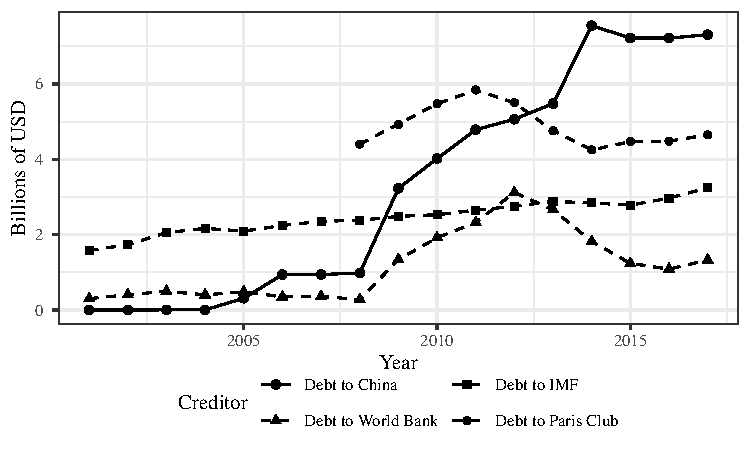
\includegraphics[width = 0.7\textwidth]{fig/sri_lanka_debt_source.pdf}
    \caption{Debt to All Creditors for Sri Lanka}
    \label{fig: sri-lanka-debt-ts}
\end{figure}